\chapter{Introduction}
\label{sec:einleitung}
The field of \emph{Robotics} have seen a tremendous development since the introduction of the term by \emph{Isaac Asimov} in 1940s. The fundamental components of robotic systems are mechanical structure, actuators, sensors and controller. Robotic systems range from simple \emph{Cartesian manipulator} to the complex \emph{Humanoids}. \emph{Industrial robots} are robots that are used in applications such as palletizing, material loading and unloading, part sorting, packaging etc. These robots usually operate in the structured environment whose geometrical or physical characteristics are known a priori. They are preprogrammed to execute the set of tasks. These robots have largely aided the automation of manufacturing processes in the industries. \emph{Mobile robots} that are used in the environments where human beings can hardly survive or be exposed to unsustainable risks are called \emph{Field robots}. These robots normally operate in the unstructured environments, where the geometry or physical characteristics are not known a priori. The mars rover \emph{Curiosity} is one such example. Locomotion in these robots is achieved either by wheels or by mechanical legs. The robots that navigate with mechanical legs are gaining importance, because they can navigate through the rugged terrain. The legged robots are biologically inspired structures equipped with six (hexapod-inspired from insects), four (quadrapod-inspired from animals) and two (biped-inspired from human) legs. The bipeds having the same kinematic structure as the humans are called \emph{Humanoids}. \emph{Toro (Torque controlled robot)} is the humanoid developed by Department of Robotics and Mechatronics at DLR. It is used as a platform to test advanced control concepts used for waling and balancing. \emph{Toro} was built as a biped walker shown in Figure \ref{fig:toro_biped}. Later in 2012 it have been equipped with the upperbody and hands and evolved into a humanoid. The present form of \emph{Toro} is shown in \ref{fig:toro_humanoid}.
\begin{figure}
	\centering
	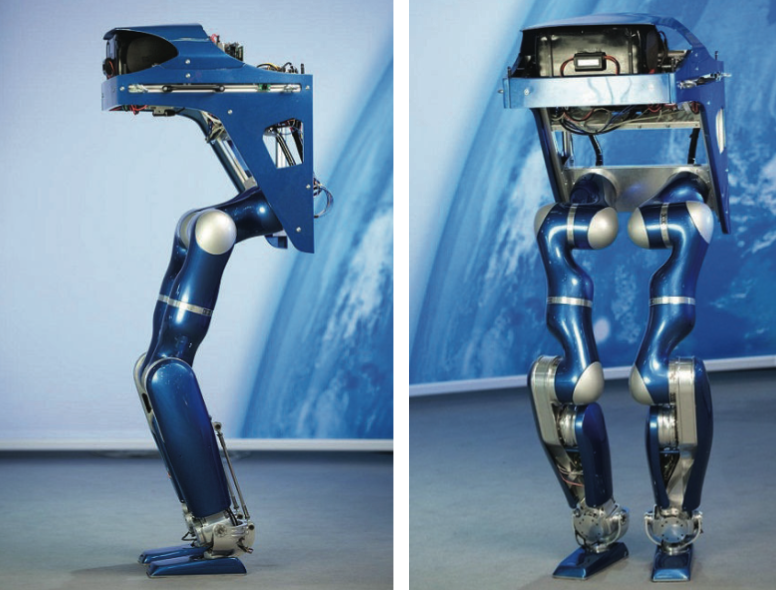
\includegraphics[scale=0.25]{Bilder/toro-biped}
	\caption{\emph{Toro} in biped form}
	\label{fig:toro_biped}
\end{figure}
\begin{figure}
\centering
	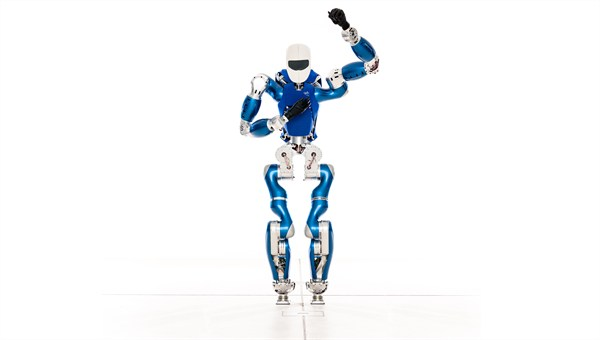
\includegraphics[trim=40mm 0mm 40mm 0mm,clip,scale=1]{Bilder/toropic}
	\caption{\emph{Toro} in humanoid form}
	\label{fig:toro_humanoid}
\end{figure}

\section{Motivation}
\begin{figure}
	\centering
	%\includegraphics[angle=-90,scale=0.65]{Bilder/walking_ctrl.pdf}
	%\pgfdeclarelayer{background}
%\pgfdeclarelayer{foreground}
%\pgfsetlayers{background,main,foreground}

% Define a few styles and constants
\tikzstyle{smallbox}=[draw, top color=white, bottom color=blue!20, text width=5em,text centered, minimum height=2.5em]
\tikzstyle{relationship} = [diamond,top color=white,bottom color=red!20,draw=red!50!black!100]
\tikzstyle{bigbox} = [smallbox,top color=white,fill=green!30,minimum height=25em,rounded corners]
\tikzstyle{input} = [coordinate]
\tikzstyle{sum} = [draw, fill=blue!20, circle, node distance=1cm]
\tikzstyle{output} = [coordinate]
\def\blockdist{3}
\def\edgedist{1.5}

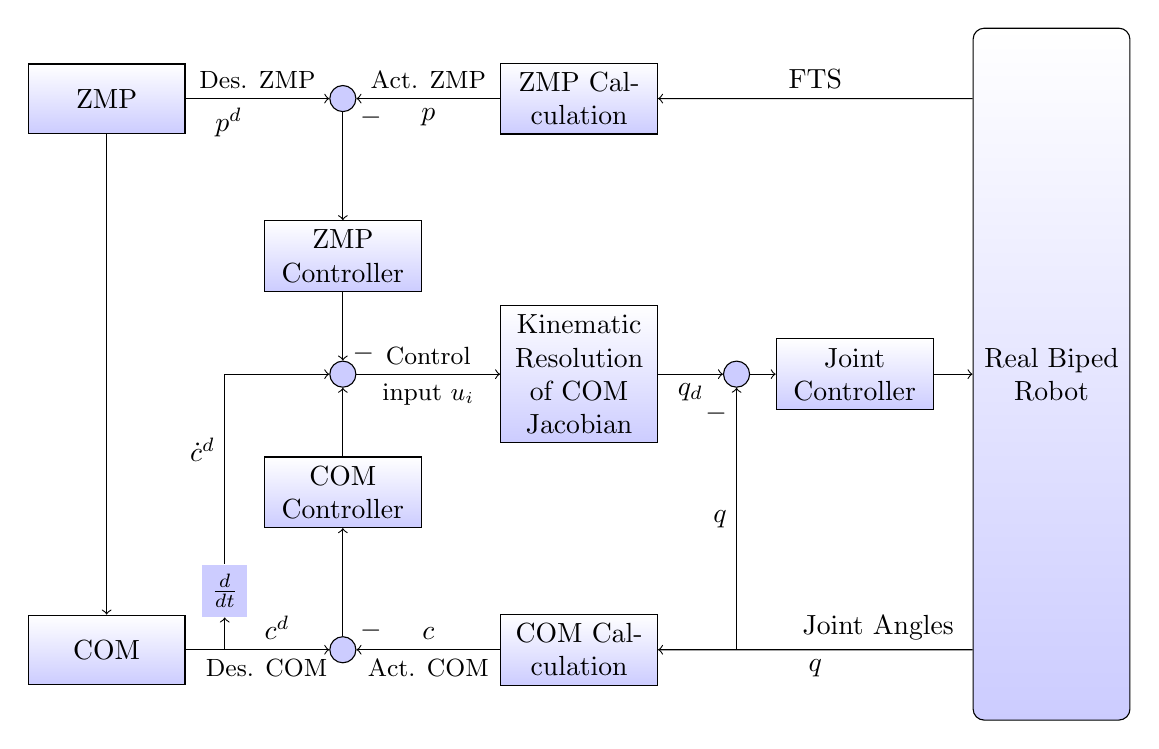
\begin{tikzpicture}[node distance=2cm]
	\node (zmp)[smallbox] {ZMP};
	\node (com) [smallbox,below of=zmp,node distance=7cm] {COM};
	\node (zmp_sum) [sum,right of=zmp,node distance=3cm]{};
	\node (zmp_ctrl) [smallbox,below of=zmp_sum,node distance=2cm]{ZMP Controller};
	\node (ctrl_sum) [sum,below of=zmp_ctrl,node distance=1.5cm]{};
	\node (kin_res) [smallbox,right of=ctrl_sum,node distance=3cm]{Kinematic Resolution of COM Jacobian};
	\node (jnt_sum) [sum,right of=kin_res,node distance=2cm]{};
	\node (jnt_msr) [input,below of=jnt_sum,node distance=3.5cm]{};
	\node (zmp_calc) [smallbox,right of=zmp_sum,node distance=3cm]{ZMP Calculation};
	\node (com_div) [output,right of=com,node distance=1.5cm]{};
	\node (dxdt) [rectangle,fill=blue!20,above of=com_div,node distance=0.75cm]{$\frac{d}{dt}$};
	\node (com_sum) [sum,below of=zmp_sum,node distance=7cm]{};
	\node (com_ctrl) [smallbox,above of=com_sum,node distance=2cm]{COM Controller};
	\node (com_calc) [smallbox,below of=zmp_calc,node distance=7cm]{COM Calculation};
	\node (jnt_ctrl) [smallbox,right of=jnt_sum,node distance=1.5cm]{Joint Controller};
	\node (robot) [bigbox,right of=jnt_ctrl,node distance=2.5cm]{Real Biped Robot};
	
	\draw [->] (zmp) --node[above,pos=0.5]{\small{Des. ZMP}}(zmp_sum)node[below,pos=0.3]{$p^d$};
	\draw [->] (zmp) --node{}(com);
	\draw [-] (com) --node{}(com_div);
	\draw [->] (com_div) --node[below,pos=0.4]{\small{Des. COM}}node[above]{$c^d$}(com_sum);
	\draw [->] (com_calc) --node[below,pos=0.5]{\small{Act. COM}}node[above,pos=0.5]{$c$}node[above,pos=0.9]{$-$}(com_sum);
	\draw [->] (com_div) --node{}(dxdt);
	\draw [->] (com_sum) --node{}(com_ctrl);
	\draw [->] (dxdt) |-node[left,pos=0.3]{$\dot c^d$}(ctrl_sum);
	\draw [->] (com_ctrl) --node{}(ctrl_sum);
	\draw [->] (zmp_ctrl) --node[right,pos=0.9]{$-$}(ctrl_sum);
	\draw [->] (ctrl_sum) --node[above,pos=0.5]{\small{Control}}node[below,pos=0.5]{\small{input }$u_i$}(kin_res);
	\draw [->] (zmp_sum) --node{}(zmp_ctrl);
	\draw [->] (zmp_calc) --node[above]{\small{Act. ZMP}}node[below]{$p$}node[below,pos=0.9]{$-$}(zmp_sum);
	\draw [->] (kin_res) --node[below]{$q_d$}(jnt_sum);
	\draw [->] (jnt_sum) --node{}(jnt_ctrl);
	\draw [->] (jnt_msr) --node[left]{$q$}node[left,pos=0.9]{$-$}(jnt_sum);
	\draw [->] (jnt_ctrl)--node{}(robot);
	\draw [->] (robot.west)+(0,3.5) --node[above]{FTS}(zmp_calc.east);
	\draw [->] (robot.west)+(0,-3.5) --node[above,pos=0.3]{Joint Angles}node[below]{$q$}(com_calc);
	
	\end{tikzpicture}

	\vspace{0.5cm}
	\caption{A walking controlled scheme of humanoid robot}
	\label{fig:walk_ctrl}
\end{figure}
% Navigating the humanoids in the unknown environments and dynamic balancing of mechanical structure demands advanced control schemes. \\
The walking control of a humanoid requires the trajectory tracking while maintaining the dynamic balance of the whole structure. The Figure \ref{fig:walk_ctrl} shows a Zero moment point (ZMP) based humanoid walking control scheme \citep{choi07}. Zero moment point is a point on the surface of the foot about which the combination of inertial forces and gravity forces does not produce any net moment. It is useful for determining the dynamic stability of the robot. The ZMP of a foot is computed from the ground reaction forces measured by the FTS [Appendix \ref{sec:zmp}]. The COM in the Figure \ref{fig:walk_ctrl} represents the center of mass of the object. In this control scheme the trajectory tracking is done by controlling the COM, and the dynamic balance is maintained by controlling the ZMP of the robot. The ZMP and COM controllers are the high level controllers that drives the Kinematic resolution of COM block which computes the desired joint angles $q_d$. The joint angles are controlled by a low level joint controller.

\paragraph{Illustartion:}    
     \begin{figure}
	    \centering
    	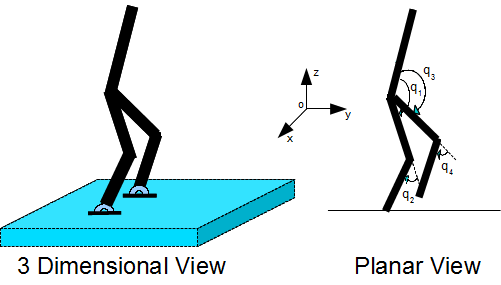
\includegraphics[scale=0.75]{Bilder/robot_flatfloor}
	    \caption{Humanoid robot standing on flat surface}	
	    \label{fig:flat_floor}
    \end{figure}
   Figure \ref{fig:flat_floor} shows a simplified two dimensional version of a humanoid robot standing on the flat surface. The COM of the robot is 
    \begin{equation}
    \label{eq:fwkin_flat}
    COM = f(q_1,q_2,q_3,q_4),
    \end{equation}
    where $f()$ is the forward kinematic function that determines the position of COM based on the joint anglse $q_i$. 
    \begin{figure}
	    \centering
    	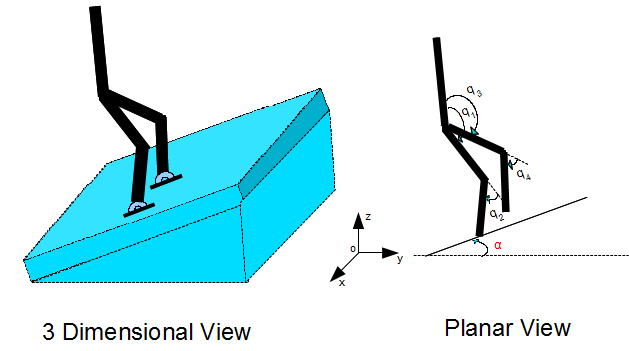
\includegraphics[scale=0.65]{Bilder/robot_slope}
	    \caption{Humanoid robot standing on a slope}	
	    \label{fig:slope}
    \end{figure}
The Figure \ref{fig:slope} shows a humanoid robot standing on the sloping surface. %In this case the COM computed by the forward kinematics function in Equation \ref{eq:fwkin_flat} will be wrong. 
%As we can see in the Figure \ref{fig:slope} there is an additional angle $\alpha$ acting between the surface of the real ground and the slope. There is no direct measurement available for this under-actuated degree of freedom. Failure to estimate this angle may lead to  tilting over an edge which might cause the robot to fall on the ground. Estimating this angle will help to achieve good balancing in the humanoid robot.
 The COM of the robot in Figure \ref{fig:slope} is given by $$COM = f(q_1,q_2,q_3,q_4,\alpha).$$  The angle $\alpha$ made by the robot with respect to the spatial frame (world coordinate frame) $O$ is not known. The computation of COM as a based on joint angles in Equation \ref{eq:fwkin_flat} will be incorrect in this case. Ignoring the angle $\alpha$ for COM computation will cause malfunctioning of the COM controller in Figure \ref{fig:walk_ctrl} and produces wrong control inputs $u_i$. The kinematic resolution of COM Jacobian block computes the desired joint angles $q_d$ assuming the robot is standing on a flat surface. When this joint trajectory executed by the controller it will cause the robot to tilt backwards. This will eventually lead to failure of the whole control scheme. This scenario motivates us to estimate the angle $\alpha$ in order to achieve robust control.  

\section{Problem Statement}
%    The focus of this thesis is estimation of under-actuated degrees of freedom of a humanoid robot.  Degrees of freedom of a robot is the number of joints present in the robot \citep{mur94}. In contrast to fixed base manipulators where the degrees of freedom is equal to number of joints in robot, the degrees of freedom of a humanoid robot is equal to sum of number of joints and degrees of freedom of a single rigid body. The under-actuated degrees of freedom of a humanoid robot are the degrees of freedom of a  rigid body.  A rigid body in three dimensional space can exhibit translational motion along \textbf{X,Y,Z} axes and rotational motion around these axes namely \emph{ roll, pitch ,yaw} as shown in Figure \ref{fig:rbody} in Chapter \ref{ch:multi_mdl}. 
	The angle $\alpha$ in Figure \ref{fig:slope} is the underactuated degree of freedom of the robot. 
% \paragraph{Underactuated degrees of freedom:}
    The term "underactuated degrees of freedom" means these degrees of freeodom are uncontrolled. They are the number of independent motions that can be exhibited by an object. For example in a two dimension (2D) space any object has 3 degrees of freedom, the object can translate along $X$ and $Y$ axes and rotate around $Z$ axis. The underactuated degrees of freedom are powered by the external forces acting on the object. For example the gravitational force makes the moon to rotate around the earth. It is not possible to directly control these degrees of freedom \citep{sab00}. In the industrial manipulators these degrees of freedom are constrained (by fixing the base to the ground), inorder to avoid complexity in control.
%%%%%%%%%%%%%%%%%%%%%%%%%%%%%%%%%%%%%%%%%%%%%%%%%%%%%%
 \begin{comment}
    \begin{figure}
    \begin{center}
    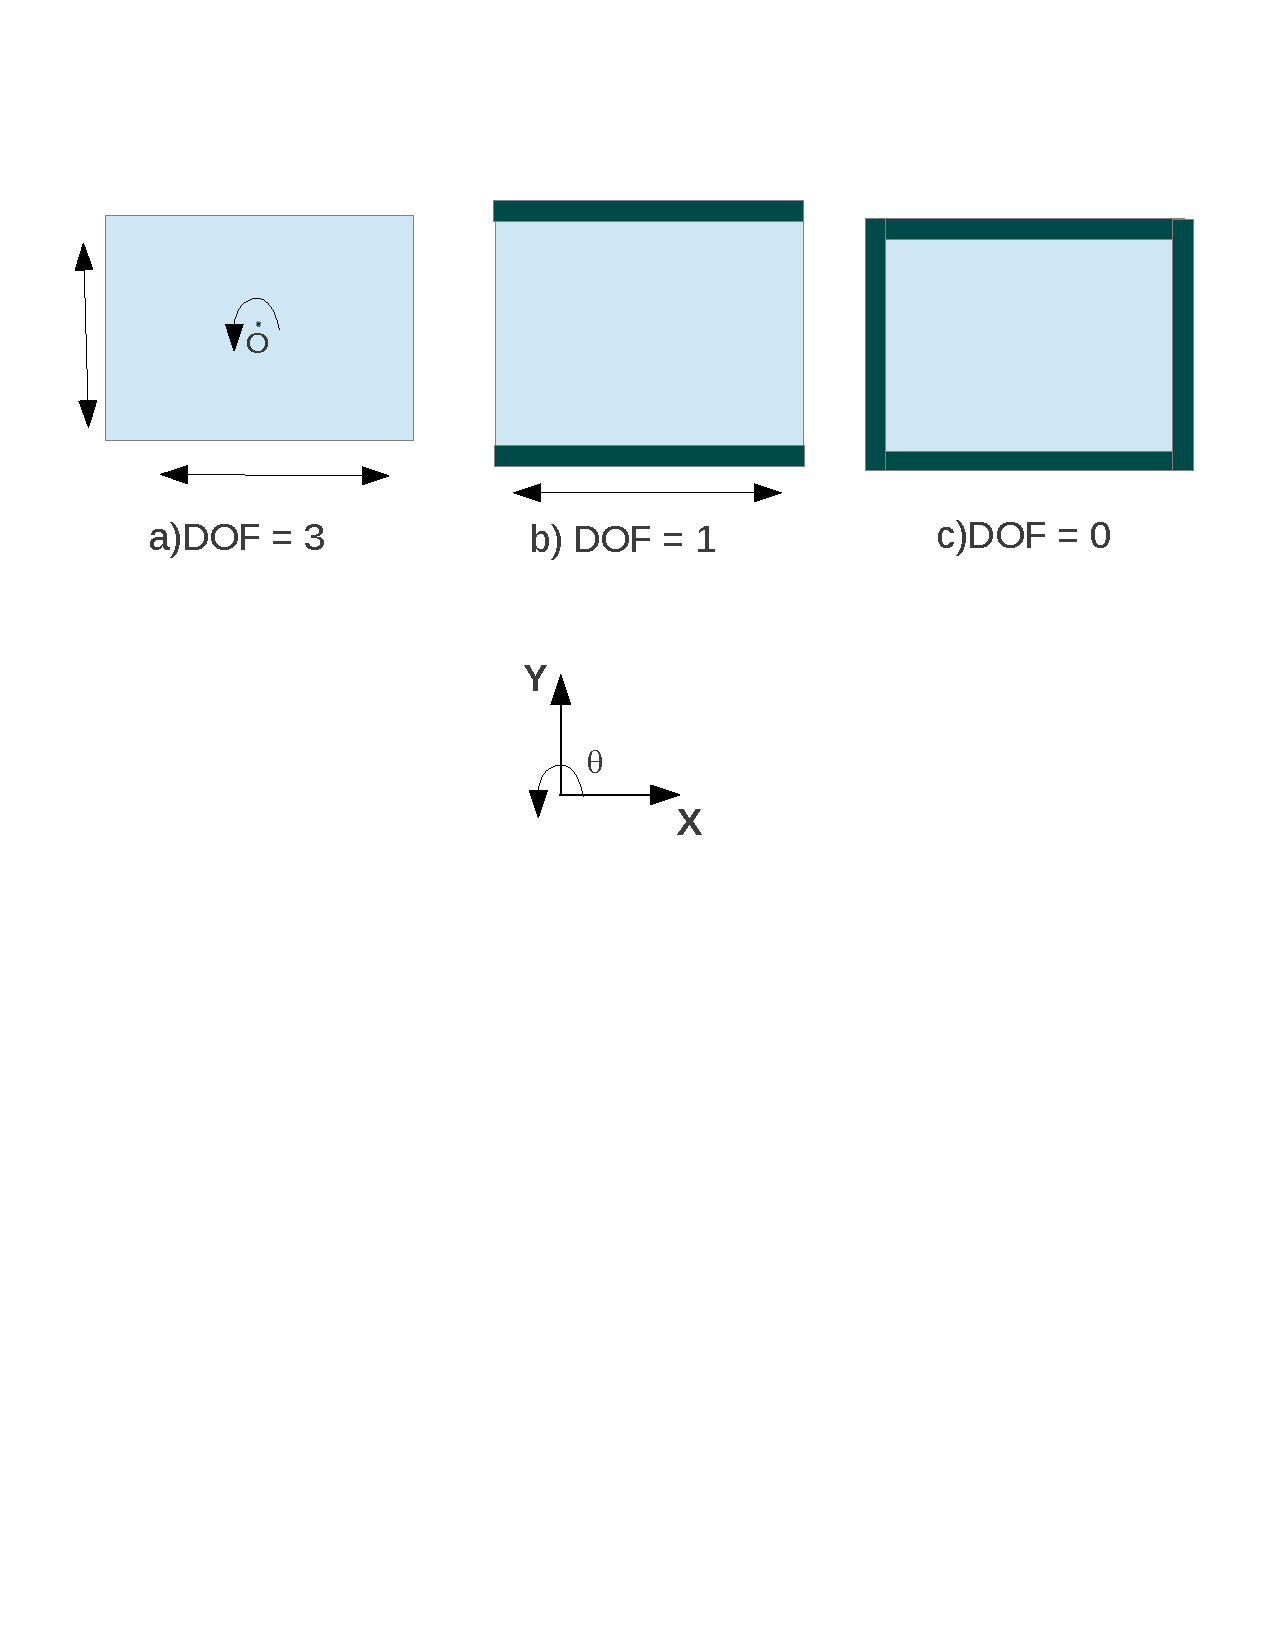
\includegraphics[trim = 10mm 130mm 10mm 20mm, scale = 0.75 ]{Bilder/dof2d.pdf}
    \caption{ Degrees of freedom of two dimensional object}
    \label{fig:dof_2d}
    \end{center}
    \end{figure}
    Figure \ref{fig:dof_2d} show how an object loses its degrees of freedom when it is constrained in 2 dimension space. In Figure \ref{fig:dof_2d} a) represents the unconstrained rectangular object free to move in space, b) represents the rectangular object constrained to move only along x axis and c) represents fully constrained rectangular object. 
    \end{comment}
%%%%%%%%%%%%%%%%%%%%%%%%%%%%%%%%%%%%%%%%%%%%%%%%%%%%%%%%%%%    
    %The ZMP of a foot is computed from the ground reaction forces measured by the FTS [Appendix \ref{sec:zmp}]. 
     
   The humanoid robots operates in a three dimensional (3D) space. The number of underactuated degrees of freedom of a 3D space is 6. 
   %When a humanoid is freely suspended (it is floating in air) it has six free degrees of freedom. But when it is constrained to its environment, the number of degrees of freedom decreases. 
   In this thesis we aim to estimate the motion of these degrees of freedom of a humanoid robot. The underactuated degrees of freedom are associated with a coordinate frame attached to the robot. In \emph{Toro} the coordinate frame is attached to the hip. As a result the state estimation problem involves estimating the motion of the hip coordinate frame. The motion parameters estimated are the position $p$, orientation $\theta$ and the body velocity $V^b$.

 \section{Methodology} 
The Kalman filter is an optimal state estimator for linear systems. The popular nonlinear extensions of Kalman filters used in practice are Extended Kalman filter(EKF) and Unscented Kalman filter(UKF). The usage of EKF for state estimation in humanoids is discussed in \citep{atk12}. \citep{bloe12} uses the EKF for state estimation in the hexapod robot. \citep{oli12} uses UKF for state estimation in humanoid robot. \citep{edg03} uses UKF for tracking the orientation of an inertial measurement unit. In this thesis the estimation problem is solved in both versions of Kalman filter. The results are compared based on accuracy of estimates and simulation time. Chapter \ref{ch:st_est} gives brief introduction to state estimation and describes the Kalman filtering algorithm. EKF and UKF algorithms are presented in Chapter \ref{ch:st_est}.

    Two different models are used for state estimation. They are the multibody system model and a simple model of  inertial measurement unit(IMU) \citep{bloe12}. The multibody system is a modelling formalism that is used to model the dynamic behaviour of a group of rigid bodies connected together to form the system. The state estimation problem using multibody system formulation is discussed in \citep{atk12}. In \citep{atk12}, the multibody system model of a simplified planar humanoid robot is used for predicting the states ahead of time. \citep{oli12} uses a multibody system model of the robot modelled using a maximal coordinate formulation scheme. The state estimation is performed separately on each link of the robot. Then the constraints due to the joints and contact are imposed on the estimates to get the true estimate of states. In this thesis, \emph{Toro} is modelled as a multibody system using minimum coordinate formulation or generalized coordinate formulation. State estimation of the multibody system involves estimation of position and velocity of the generalized coordinates. For instance, the model of \emph{Toro} have 31 generalized coordinates. The result of estimation problem will be 31 positions and 31 velocities of the generalized coordinates. Chapter \ref{ch:multi_mdl} deals with the modelling of multibody systems and its implementation in Kalman filtering algorithm. 
    
    A simplified motion model of IMU is discussed in \cite{bloe12}. In this paper, the EKF is used as sensor fusion algorithm for fusing IMU information with the kinematics of the hexapod. \citep{vis12} describes about an on-board odometry filter. The EKF is used to fuse the IMU motion model with the visual odometry and the kinematic odometry. The odometry filter is combined with vision based SLAM to obtain improved estimate of the motion model. An approach similar to \cite{bloe12} is implemented for humanoid robots. It is dealt in Chapter \ref{ch:simp_mdl}. The state estimation using this model involves predicting the position, orientation, translational velocity of the IMU sensor ahead of time. The position, orientation estimated are the under-actuated degrees of freedom and of the humanoid robot. This predicted states are updated by the kinematic information about the leg. State estimation using this model is more simpler than the multibody system. It is practically implemented on \emph{Toro}.
